\documentclass[12pt,titlepage]{article}
\usepackage[margin=1.25in]{geometry}
\usepackage{graphicx,amsmath,blindtext}

%% Variables definition
\newcommand{\vSubject}{Artificial Intelligence}
\newcommand{\vSubtitle}{Fundamentals Use Case for AI}
\newcommand{\vName}{Dicha Zelianivan Arkana}
\newcommand{\vNIM}{2241720002}
\newcommand{\vClass}{1i}
\newcommand{\vDepartment}{Information Technology}
\newcommand{\vStudyProgram}{D4 Informatics Engineering}

%% [START] Tikz related stuff
\usepackage{tikz}
\usetikzlibrary{svg.path,calc,shapes.geometric,shapes.misc}
\tikzstyle{terminator} = [rectangle, draw, text centered, rounded corners = 1em, minimum height=2em]
\tikzstyle{preparation} = [chamfered rectangle, chamfered rectangle sep=0.75em, draw, text centered, minimum height = 2em]
\tikzstyle{process} = [rectangle, draw, text centered, minimum height=2em]
\tikzstyle{decision} = [diamond, aspect=2, draw, text centered, minimum height=2em]
\tikzstyle{data}=[trapezium, draw, text centered, trapezium left angle=60, trapezium right angle=120, minimum height=2em]
\tikzstyle{connector} = [line width=0.25mm,->]
%% [END] Tikz related stuff

%% [START] Fancy header related stuff
\usepackage{fancyhdr}
\pagestyle{fancy}
\setlength{\headheight}{15pt} % compensate fancyhdr style
\fancyhead{}
\fancyfoot{}
\fancyfoot[L]{\thepage}
\fancyfoot[R]{\textit{\vSubject - \vSubtitle}}
\renewcommand{\footrulewidth}{0.4pt}% default is 0pt, overline for footer
%% [END] Fancy header related stuff

%% [START] Custom tabular command related stuff
\usepackage{tabularx}
\newcommand{\details}[2]{
    #1 & #2  \\
}
%% [END] Custom tabular command related stuff

%% [START] Figure related stuff
\newcommand{\image}[3][1]{
    \begin{figure}[h]
        \centering
        \includegraphics[#1]{#2}
        \caption{#3}
        \label{#3}
    \end{figure}
}
%% [END] Figure related stuff

\begin{document}
\begin{titlepage}
    \centering
    \vfill
    {\bfseries\LARGE
        \vSubject\\
        \vskip0.25cm
        \vSubtitle
    }
    \vfill
    
\includegraphics[width=6cm]{images/polinema-logo.png}
    \vfill
    {
        \textbf{Name}\\
        \vName\\
        \vskip0.5cm
        \textbf{NIM}\\
        \vNIM\\
        \vskip0.5cm
        \textbf{Class}\\
        \vClass\\
        \vskip0.5cm
        \textbf{Department}\\
        \vDepartment\\
        \vskip0.5cm
        \textbf{Study Program}\\
        \vStudyProgram
    }
\end{titlepage}

\tableofcontents
\pagebreak

\section{Questions}
\subsection{What happens if an AI became so evolved that it became conscious? Should it be given rights?}
If at some point the technology of Artificial Intelligence has reached that point, I think it's fair that we give them
the rights to exist, just not on the same level as humans. A rights with their own rules and capabilities.
We can't just give them the same rights as humans because they are not humans. 
They are just a bunch of codes that can think and act like humans.
They are not born like humans, they are created by humans.

\subsection{If a Robot replaces a human, should companies be required to continue paying payroll tax for that displaced worker?}
I think it's not fair for them to get paid because they're not doing anything. Also I personally don't think that it's
good to pay someone for doing nothing, for their own good. It's better to give them a new job that they can do, because I don't think
literally eveything can be replaced by AI.

\subsection{Will we get to a point where computers are doing everything, and if so, how will we adapt to this; how will we spend our time?}
I do think we can reach that point, but I don't think it will be in the near future either. Although the chance of it happening is very unlikely.

I think we will adapt to this by doing something else that we can do, like doing something that we like, or something that we can't do with AI.
We as a human being will have desires that can't be fulfilled by AI, and that's what we will do, such as interacting with
other human beings, or doing something that we like, even if it's not productive.

There are the good and the bad side of this. The good side is that we can do something that we like, no longer need to think about productivity and things that makes us stressed.
The bad side is that we will become lazy, and we will at some point lose our purpose in life. 

\subsection{Worse yet, does the technology enable a few individuals to control all resources? Will a universal income society emerge in which individuals can pursue their own interests? Or will the displaced masses live in poverty?}
I think it highly depends on the human desires. If we reached a point where a Universal Basic Income can be achieved, then everyone will be "wealthy" in a sense.
Despite this situation, there will always be someone who wants more, and that's where the problem will arise. The problem will be the same as the problem that we have now,
the problem of inequality.

\pagebreak

\section{Artificial Intelligence Use Case Infographic}
\begin{figure}[h]
    \centering
    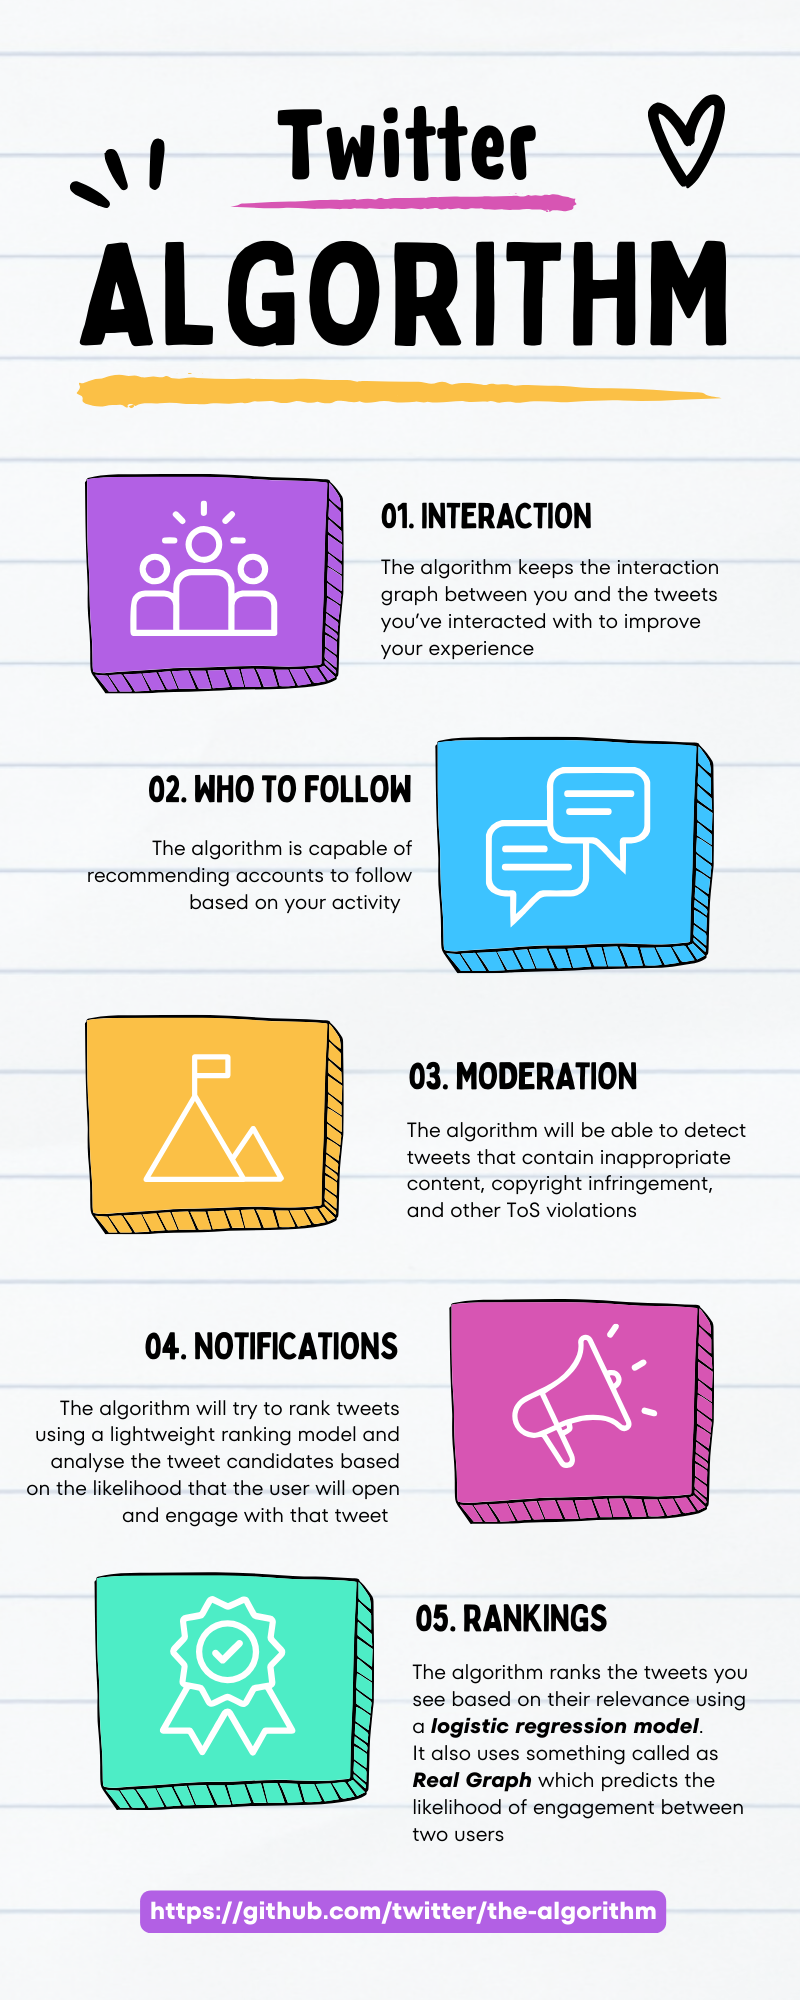
\includegraphics[height=0.6\pdfpageheight]{./images/twitter-algorithm-infographic.png}
\end{figure}

\end{document}

